% Options for packages loaded elsewhere
\PassOptionsToPackage{unicode}{hyperref}
\PassOptionsToPackage{hyphens}{url}
%
\documentclass[
  man]{apa6}
\usepackage{amsmath,amssymb}
\usepackage{iftex}
\ifPDFTeX
  \usepackage[T1]{fontenc}
  \usepackage[utf8]{inputenc}
  \usepackage{textcomp} % provide euro and other symbols
\else % if luatex or xetex
  \usepackage{unicode-math} % this also loads fontspec
  \defaultfontfeatures{Scale=MatchLowercase}
  \defaultfontfeatures[\rmfamily]{Ligatures=TeX,Scale=1}
\fi
\usepackage{lmodern}
\ifPDFTeX\else
  % xetex/luatex font selection
\fi
% Use upquote if available, for straight quotes in verbatim environments
\IfFileExists{upquote.sty}{\usepackage{upquote}}{}
\IfFileExists{microtype.sty}{% use microtype if available
  \usepackage[]{microtype}
  \UseMicrotypeSet[protrusion]{basicmath} % disable protrusion for tt fonts
}{}
\makeatletter
\@ifundefined{KOMAClassName}{% if non-KOMA class
  \IfFileExists{parskip.sty}{%
    \usepackage{parskip}
  }{% else
    \setlength{\parindent}{0pt}
    \setlength{\parskip}{6pt plus 2pt minus 1pt}}
}{% if KOMA class
  \KOMAoptions{parskip=half}}
\makeatother
\usepackage{xcolor}
\usepackage{graphicx}
\makeatletter
\def\maxwidth{\ifdim\Gin@nat@width>\linewidth\linewidth\else\Gin@nat@width\fi}
\def\maxheight{\ifdim\Gin@nat@height>\textheight\textheight\else\Gin@nat@height\fi}
\makeatother
% Scale images if necessary, so that they will not overflow the page
% margins by default, and it is still possible to overwrite the defaults
% using explicit options in \includegraphics[width, height, ...]{}
\setkeys{Gin}{width=\maxwidth,height=\maxheight,keepaspectratio}
% Set default figure placement to htbp
\makeatletter
\def\fps@figure{htbp}
\makeatother
\ifLuaTeX
  \usepackage{luacolor}
  \usepackage[soul]{lua-ul}
\else
  \usepackage{soul}
\fi
\setlength{\emergencystretch}{3em} % prevent overfull lines
\providecommand{\tightlist}{%
  \setlength{\itemsep}{0pt}\setlength{\parskip}{0pt}}
\setcounter{secnumdepth}{-\maxdimen} % remove section numbering
% Make \paragraph and \subparagraph free-standing
\makeatletter
\ifx\paragraph\undefined\else
  \let\oldparagraph\paragraph
  \renewcommand{\paragraph}{
    \@ifstar
      \xxxParagraphStar
      \xxxParagraphNoStar
  }
  \newcommand{\xxxParagraphStar}[1]{\oldparagraph*{#1}\mbox{}}
  \newcommand{\xxxParagraphNoStar}[1]{\oldparagraph{#1}\mbox{}}
\fi
\ifx\subparagraph\undefined\else
  \let\oldsubparagraph\subparagraph
  \renewcommand{\subparagraph}{
    \@ifstar
      \xxxSubParagraphStar
      \xxxSubParagraphNoStar
  }
  \newcommand{\xxxSubParagraphStar}[1]{\oldsubparagraph*{#1}\mbox{}}
  \newcommand{\xxxSubParagraphNoStar}[1]{\oldsubparagraph{#1}\mbox{}}
\fi
\makeatother
% definitions for citeproc citations
\NewDocumentCommand\citeproctext{}{}
\NewDocumentCommand\citeproc{mm}{%
  \begingroup\def\citeproctext{#2}\cite{#1}\endgroup}
\makeatletter
 % allow citations to break across lines
 \let\@cite@ofmt\@firstofone
 % avoid brackets around text for \cite:
 \def\@biblabel#1{}
 \def\@cite#1#2{{#1\if@tempswa , #2\fi}}
\makeatother
\newlength{\cslhangindent}
\setlength{\cslhangindent}{1.5em}
\newlength{\csllabelwidth}
\setlength{\csllabelwidth}{3em}
\newenvironment{CSLReferences}[2] % #1 hanging-indent, #2 entry-spacing
 {\begin{list}{}{%
  \setlength{\itemindent}{0pt}
  \setlength{\leftmargin}{0pt}
  \setlength{\parsep}{0pt}
  % turn on hanging indent if param 1 is 1
  \ifodd #1
   \setlength{\leftmargin}{\cslhangindent}
   \setlength{\itemindent}{-1\cslhangindent}
  \fi
  % set entry spacing
  \setlength{\itemsep}{#2\baselineskip}}}
 {\end{list}}
\usepackage{calc}
\newcommand{\CSLBlock}[1]{\hfill\break\parbox[t]{\linewidth}{\strut\ignorespaces#1\strut}}
\newcommand{\CSLLeftMargin}[1]{\parbox[t]{\csllabelwidth}{\strut#1\strut}}
\newcommand{\CSLRightInline}[1]{\parbox[t]{\linewidth - \csllabelwidth}{\strut#1\strut}}
\newcommand{\CSLIndent}[1]{\hspace{\cslhangindent}#1}
\ifLuaTeX
\usepackage[bidi=basic]{babel}
\else
\usepackage[bidi=default]{babel}
\fi
\babelprovide[main,import]{english}
% get rid of language-specific shorthands (see #6817):
\let\LanguageShortHands\languageshorthands
\def\languageshorthands#1{}
% Manuscript styling
\usepackage{upgreek}
\captionsetup{font=singlespacing,justification=justified}

% Table formatting
\usepackage{longtable}
\usepackage{lscape}
% \usepackage[counterclockwise]{rotating}   % Landscape page setup for large tables
\usepackage{multirow}		% Table styling
\usepackage{tabularx}		% Control Column width
\usepackage[flushleft]{threeparttable}	% Allows for three part tables with a specified notes section
\usepackage{threeparttablex}            % Lets threeparttable work with longtable

% Create new environments so endfloat can handle them
% \newenvironment{ltable}
%   {\begin{landscape}\centering\begin{threeparttable}}
%   {\end{threeparttable}\end{landscape}}
\newenvironment{lltable}{\begin{landscape}\centering\begin{ThreePartTable}}{\end{ThreePartTable}\end{landscape}}

% Enables adjusting longtable caption width to table width
% Solution found at http://golatex.de/longtable-mit-caption-so-breit-wie-die-tabelle-t15767.html
\makeatletter
\newcommand\LastLTentrywidth{1em}
\newlength\longtablewidth
\setlength{\longtablewidth}{1in}
\newcommand{\getlongtablewidth}{\begingroup \ifcsname LT@\roman{LT@tables}\endcsname \global\longtablewidth=0pt \renewcommand{\LT@entry}[2]{\global\advance\longtablewidth by ##2\relax\gdef\LastLTentrywidth{##2}}\@nameuse{LT@\roman{LT@tables}} \fi \endgroup}

% \setlength{\parindent}{0.5in}
% \setlength{\parskip}{0pt plus 0pt minus 0pt}

% Overwrite redefinition of paragraph and subparagraph by the default LaTeX template
% See https://github.com/crsh/papaja/issues/292
\makeatletter
\renewcommand{\paragraph}{\@startsection{paragraph}{4}{\parindent}%
  {0\baselineskip \@plus 0.2ex \@minus 0.2ex}%
  {-1em}%
  {\normalfont\normalsize\bfseries\itshape\typesectitle}}

\renewcommand{\subparagraph}[1]{\@startsection{subparagraph}{5}{1em}%
  {0\baselineskip \@plus 0.2ex \@minus 0.2ex}%
  {-\z@\relax}%
  {\normalfont\normalsize\itshape\hspace{\parindent}{#1}\textit{\addperi}}{\relax}}
\makeatother

\makeatletter
\usepackage{etoolbox}
\patchcmd{\maketitle}
  {\section{\normalfont\normalsize\abstractname}}
  {\section*{\normalfont\normalsize\abstractname}}
  {}{\typeout{Failed to patch abstract.}}
\patchcmd{\maketitle}
  {\section{\protect\normalfont{\@title}}}
  {\section*{\protect\normalfont{\@title}}}
  {}{\typeout{Failed to patch title.}}
\makeatother

\usepackage{xpatch}
\makeatletter
\xapptocmd\appendix
  {\xapptocmd\section
    {\addcontentsline{toc}{section}{\appendixname\ifoneappendix\else~\theappendix\fi: #1}}
    {}{\InnerPatchFailed}%
  }
{}{\PatchFailed}
\makeatother
\keywords{graphical representation, iconicity, analogy, symbol, communication, emerging literacy\newline\indent Word count: Child Development Max 40 pages // PNAS 1,500–2,000 words}
\DeclareDelayedFloatFlavor{ThreePartTable}{table}
\DeclareDelayedFloatFlavor{lltable}{table}
\DeclareDelayedFloatFlavor*{longtable}{table}
\makeatletter
\renewcommand{\efloat@iwrite}[1]{\immediate\expandafter\protected@write\csname efloat@post#1\endcsname{}}
\makeatother
\usepackage{lineno}

\linenumbers
\usepackage{csquotes}
\ifLuaTeX
  \usepackage{selnolig}  % disable illegal ligatures
\fi
\usepackage{bookmark}
\IfFileExists{xurl.sty}{\usepackage{xurl}}{} % add URL line breaks if available
\urlstyle{same}
\hypersetup{
  pdftitle={Young children's spontaneous comprehension of symbol-object-relationships in the graphic domain},
  pdfauthor={Gregor Kachel1, Daniel Haun2, \& Manuel Bohn1},
  pdflang={en-EN},
  pdfkeywords={graphical representation, iconicity, analogy, symbol, communication, emerging literacy},
  hidelinks,
  pdfcreator={LaTeX via pandoc}}

\title{Young children's spontaneous comprehension of symbol-object-relationships in the graphic domain}
\author{Gregor Kachel\textsuperscript{1}, Daniel Haun\textsuperscript{2}, \& Manuel Bohn\textsuperscript{1}}
\date{}


\shorttitle{Comprehension of symbol-object-relationships}

\authornote{

\emph{Ethics, consent and conflict of interest}: This study confirms with recognized standards (e.g.~the Declaration of Helsinki) and was approved by an internal ethics committee at the Max-Planck-Institute for Evolutionary Anthropology. Informed consent has been obtained from all participants. The authors declare no conflict of interest.

\emph{Acknowledgments}: We are thankful to Susanne Mauritz for her help in the organization of the study and to Valerie Jurgenson and Cynthia Pones for help with data collection. We would like to thank Anne Deiglmayr for hosting this project in her research group and for her continuous support. Finally, we are very thankful to all parents and children participating in the study. Gregor Kachel was supported by the German Research Foundation (Deutsche Forschungsgemeinschaft) under project number 429220405.

The authors made the following contributions. Gregor Kachel: Conceptualization, Funding Acquisition, Project Administration, Investigation, Methodology, Data Curation, Formal Analysis, Visualization, Writing - Original Draft Preparation, Writing - Review \& Editing; Daniel Haun: Resources, Writing - Review \& Editing; Manuel Bohn: Methodology, Software, Formal Analysis, Validation, Writing - Review \& Editing, Supervision.

Correspondence concerning this article should be addressed to Gregor Kachel, Universitätsallee 1, C1.008a, 21335 Lüneburg. E-mail: \href{mailto:gregor.kachel@leuphana.de}{\nolinkurl{gregor.kachel@leuphana.de}}

}

\affiliation{\vspace{0.5cm}\textsuperscript{1} Leuphana University\\\textsuperscript{2} Max-Planck-Institute for Evolutionary Anthropology}

\abstract{%
One or two sentences providing a \textbf{basic introduction} to the field, comprehensible to a scientist in any discipline.
Two to three sentences of \textbf{more detailed background}, comprehensible to scientists in related disciplines.
One sentence clearly stating the \textbf{general problem} being addressed by this particular study.
One sentence summarizing the main result (with the words ``\textbf{here we show}'' or their equivalent).
Two or three sentences explaining what the \textbf{main result} reveals in direct comparison to what was thought to be the case previously, or how the main result adds to previous knowledge.
One or two sentences to put the results into a more \textbf{general context}.
Two or three sentences to provide a \textbf{broader perspective}, readily comprehensible to a scientist in any discipline. !Abstract must be less then 120words!
}



\begin{document}
\maketitle

\section{Introduction}\label{introduction}

\st{Lorem ipsum dolor sit amet, consetetur sadipscing elitr, sed diam nonumy eirmod tempor invidunt ut labore et dolore magna aliquyam erat, sed diam voluptua. At vero eos et accusam et justo duo dolores et ea rebum. Stet clita kasd gubergren, no sea takimata sanctus est Lorem ipsum dolor sit amet. Lorem ipsum dolor sit amet, consetetur sadipscing elitr, sed diam nonumy eirmod tempor invidunt ut labore et dolore magna aliquyam erat, sed diam voluptua. At vero eos et accusam et justo duo dolores et ea rebum. Stet clita kasd gubergren, no sea takimata sanctus est Lorem ipsum dolor sit amet.}

Preschoolers invent and comprehend iconic gestures spontaneously (Bohn, Kachel, \& Tomasello, 2019).

\emph{Children's understanding of graphical representations}.
\st{Lorem ipsum dolor sit amet, consetetur sadipscing elitr, sed diam nonumy eirmod tempor invidunt ut labore et dolore magna aliquyam erat, sed diam voluptua. At vero eos et accusam et justo duo dolores et ea rebum. Stet clita kasd gubergren, no sea takimata sanctus est Lorem ipsum dolor sit amet. Lorem ipsum dolor sit amet, consetetur sadipscing elitr, sed diam nonumy eirmod tempor invidunt ut labore et dolore magna aliquyam erat, sed diam voluptua. At vero eos et accusam et justo duo dolores et ea rebum. Stet clita kasd gubergren, no sea takimata sanctus est Lorem ipsum dolor sit amet.}

\emph{This Paper}.
\st{Lorem ipsum dolor sit amet, consetetur sadipscing elitr, sed diam nonumy eirmod tempor invidunt ut labore et dolore magna aliquyam erat, sed diam voluptua. At vero eos et accusam et justo duo dolores et ea rebum. Stet clita kasd gubergren, no sea takimata sanctus est Lorem ipsum dolor sit amet. Lorem ipsum dolor sit amet, consetetur sadipscing elitr, sed diam nonumy eirmod tempor invidunt ut labore et dolore magna aliquyam erat, sed diam voluptua. At vero eos et accusam et justo duo dolores et ea rebum. Stet clita kasd gubergren, no sea takimata sanctus est Lorem ipsum dolor sit amet. For the first time, the studies contributing to this paper investigate children's understanding of xxx.}

\emph{Hypotheses}. \st{Lorem ipsum dolor sit amet, consetetur sadipscing elitr, sed diam nonumy eirmod tempor invidunt ut labore et dolore magna aliquyam erat, sed diam voluptua. At vero eos et accusam et justo duo dolores et ea rebum. Stet clita kasd gubergren, no sea takimata sanctus est Lorem ipsum dolor sit amet. Lorem ipsum dolor sit amet, consetetur sadipscing elitr, sed diam nonumy eirmod tempor invidunt ut labore et dolore magna aliquyam erat, sed diam voluptua. At vero eos et accusam et justo duo dolores et ea rebum. Stet clita kasd gubergren, no sea takimata sanctus est Lorem ipsum dolor sit amet.}

\section{Methods}\label{methods}

All three studies presented here share the same methods and analyses. For convenience, common aspects of the procedure, participant recruiting and stimulus design are reported first before discussing the individual studies respectively.

\subsection{General Methods}\label{general-methods}

\subsubsection{Setup and Data Collection}\label{setup-and-data-collection}

In order to trace the development of children's symbolic competence continuously across the preschool years, data collection aimed at testing two children per month of age between the third and the seventh birthday for a total 96 participants while euqally balancing male and female participants. As children participated on the basis of availability and data collection was done by several experimenter teams visiting different institutions in parallel, the resulting final samples slightly exceed this preregistered minimum sample size. The final sample approximate an equal distribution of male and female participants and
while aligning with conventions in the field, by providing at least 24 participants per condition and year of age.

All participants were recruited in \textbf{MASKED FOR REVIEW}, a medium-sized middle-European city, and came from a predominantly white population of middle to high income families. They were contacted via a database of participants for child development studies to which their parents had voluntarily signed up. Children were tested in day- and afterschoolcare for the most part, and occasionally in the lab or at home. The studies were reviewed and approved by an internal ethics committee at the \textbf{MASKED FOR REVIEW}. Data collection took place from June 2022 to February 2023.

During test sessions, one child and an experimenter sat down together to play a picture-book-style hiding game presented on a touch-screen laptop. Verbal instructions were played back by the experimental script. Experimenters supervised children during data collection an assisted with a fixed set of verbal prompts when necessary. Test sessions always took place in a quiet separate room. See figure \ref{fig:figure-setup} for an illustration of the setup.



\begin{figure}

{\centering 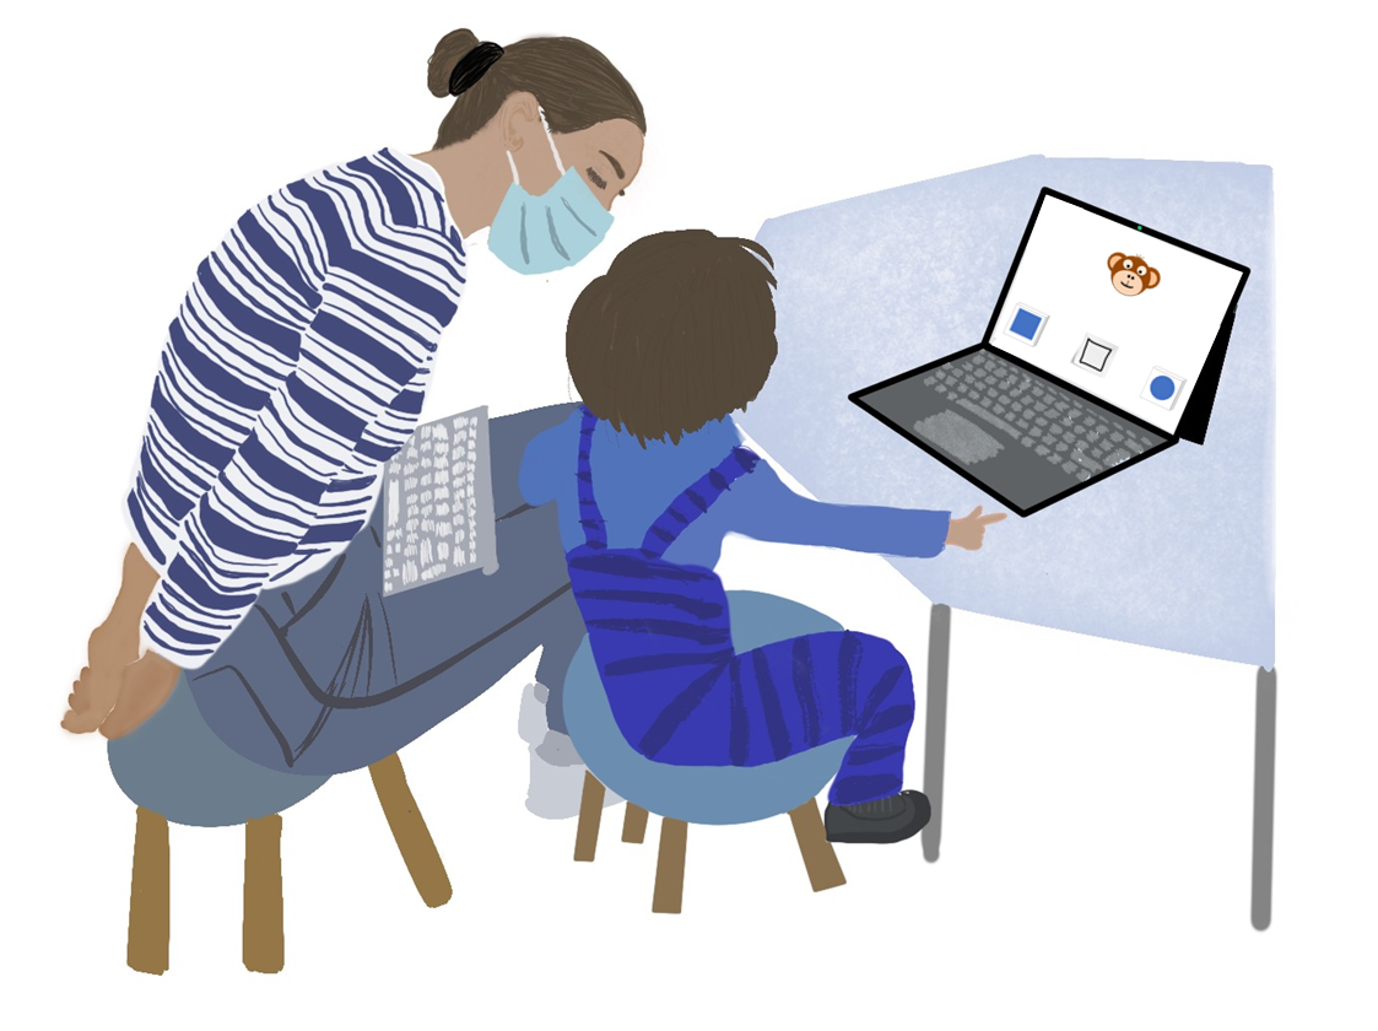
\includegraphics{../illustrations/Symlit_Rep_Setup_fromarrows} 

}

\caption{Illustration of setup. Experimenters were sitting behind the children in order to not distract them from the task and supervised data collection.}\label{fig:figure-setup}
\end{figure}

\subsubsection{Procedure}\label{procedure}

\emph{Familiarization}. Experimenters invited children to join a hiding game and to follow the narration of the story. First, the presentation introduced a cartoon monkey. This character then placed two barriers on the bottom left and right side of the screen. After holding up a banana, one of the barriers was lifted, the banana was placed there and the barrier was lowered to conceal the banana. Children were now prompted to touch the hiding place and in doing so the barrier of their choice was lifted to reveal the banana if they chose correctly. Hence to succeed here, children solely had to remember where the item went and touch this part of the screen after a few seconds. The experimental script provided immediate feedback upon children's choice (``yes, great job!''; ``No, that's not it. Let's try again!'') during the familiarization. To ensure that children were familiar with the goal of the game and the touch interface, they first had to complete a set of four to eight familiarization trials with a success rate of 75\%. In case a child did not reply correctly in three out of four trials, another four familiarization trials were provided. If the child was correct in six out of eight trials, she was included in the main sample. Children that did not succeed during familiarization were allowed to participate but their data was not submitted to analysis. These children are reported below as failing the familiarization phase.

\emph{Test phase}. The main phase of the study commenced with announcing that the cartoon character had an idea for a new game. The narration conveyed that children were not allowed to see where the banana would be hidden, but that the monkey would help them find it. Hence, the cartoon character was established as a partner in a cooperative coordination game. The hiding sequence was identical to the familiarization phase, however the placement of the banana was concealed by a barrier over the lower half of the screen and the two hiding places displayed different graphical shapes in the same colour. The monkey then held up piece of paper and a pencil. Pencil movement and a short scribble sound indicated that the monkey was drawing something. Children were reminded that the monkey was going to help them. Children were now prompted with the phrase ``Where is the banana?'' and the monkey's drawing was placed in the center between the two barriers. The drawing now served as a cue to guide children's choice. In the most basic experimental condition in study one, each hiding places, for example, showed either a solid blue circle or square and the paper displayed a simple outline drawing of either shape. Here, the drawing was a direct representation of the target shape. Crucially, however, children received only neutral feedback upon making a choice (``Ah, thank you'') and there was no reveal animation. The game simply continued with the next round in which two new hiding places with different shapes were displayed, and hiding sequence was repeated as before.

Except for the geometric shapes displayed on the hiding places and the respective drawing, the experimental representation was identical for all test trials. A single trial lasted roughly 30 to 60 seconds, depending on how swiftly children chose. Each study presented four different experimental conditions with four trials each in a blocked order for a maximum of 16 test trials. Children occasionally wished to stop before completing all trials, resulting in minor deviations of the total number of trials per condition that are submitted to analyses. Children that did not complete a minimum of eight test trials were not submitted to analysis and are reported below. The entire test session lasted about 12 minutes.

\subsubsection{Stimuli and Experimental Manipulations}\label{stimuli-and-experimental-manipulations}

Description of cues and targets and maybe how they were created.

For an illustration of the stimuli and example presentations, please see supplementary materials sections XX and XX.

\subsubsection{Data Handling and Analyses}\label{data-handling-and-analyses}

Participant choices were recorded by the experimental script and directly coded as correct or incorrect. Exclusions of data were solely made on the level of participants with regard to the exclusion criteria reported above. The analyses modeled participants' binary choices to predict the probability of children interpreting the cues correctly and to model how this probability would change as a function of their age. Logistic Bayesian generalized linear mixed models (GLMM) fitted children's responses (0/1) as a function of their age, the experimental condition and an interaction between trial and condition. Trial and sex were included as fixed effects to be controlled for. Trial number was added as a random slope within subject. To evaluate the relevance of age and condition for children's performance, a full model was compared with a reduced model lacking the interaction of age and task by using WAIC scores and weights (McElreath, 2016). Furthermore, model estimates were inspected for the different predictors (including their 95\% Credible Interval (CrI)). In each study, the most simple condition was set as the reference level within conditions. All Bayesian models used default priors and were run in Stan (\url{http://mc-stan.org/}) via the function brm of the package brms (Bürkner, 2017).

To answer the main research question of when children performed above chance in any of the study's conditions, we use the models to predict the developmental trajectory (with 95\% CrI) for each condition (expected values of the posterior predicted dist via fct fitted). The criterion for settling when children passed criterion as a group was the point at which the 95\% CrI for a particular trajectory did no longer overlap with a midline demarcating the 50\% chance level.

To further explore the data, participants were binned according to their age in years. To test whether group-level performance was above chance in all experimental groups, we used two-tailed one-sample t-tests with the chance level set to .5. We provide Cohen's d as a standardized effect size for significance testing (computed via the function \texttt{cohensD}).

\subsection{Study 1}\label{study-1}

\subsubsection{Participants}\label{participants}

A sample of 106 children (M = 59.18 months, SD = 13.58 months, range 36 - 83 months; 51 female) participated in study 1. In addition, 22 children (11 female) were tested but excluded from analysis for not succeeding during familiarization (N = 13), for not completing at least eight out of 16 test trials (N = 1), or due to being fussy (N = 2). For 4 children, experimenters only learned during testing that children were not fluent enough in German to participate as their families had only recently migrated. Finally, 2 children had to be excluded due to technical issues. For a graphical and tabular overview of participants and exclusions across all three studies presented here, please see Appendix A.

\subsubsection{Stimuli}\label{stimuli}

\subsubsection{Analyses}\label{analyses}

A total of XX trials (\emph{Representation}: ; \emph{Pars Pro Toto}: ; \emph{Simple Form Analogy}: ; \emph{Complex Form Analogy}: ) from XX participants were submitted for analysis. The full model notation was \('correct~condition*z.age+z.trial+sex+(z.trial|subid)'\). In addition, a null model lacking the interaction of condition and age (\('correct~condition+z.age+z.trial+sex+(z.trial|subid)'\)) was fitted.

\subsubsection{Notes}\label{notes}

\begin{itemize}
\tightlist
\item
  deviation from preregistration
\item
  elpd\_diff ist neu und zusätzlich
\item
  most simple condition als reference \ldots warum
\item
  bezeichnung output fitted function --\textgreater{} wie macht brms die confidence intervalle um die mittelwerte --\textgreater{}
\item
  ``expected value of the posterior predicted distribution''
\end{itemize}

\subsubsection{Results}\label{results}

ALL NUMBERS FROM MODEL CHECKS GO TO SUPPL
Posterior predictive checks for both models indicated excellent fit of observed data and model predictions. Rhat values in both models were equal to one, indicating convergence across all chains. Effective sample sizes for all fixed effects in the full model (Bulk ESS, mean = 2555, range 1760 - 3766) and the null model (Bulk ESS, mean = 2253, range 1706 - 3444) were \textgreater{} 1000, indicating reliable posterior estimations.

Comparing models using weights based on the Widely Applicable Information Criterion (WAIC) yielded 76.06\% of the model weight for the full model, and 23.94\% for the null model. Hence, the full model generally has a higher probability of making accurate predictions. Directly comparing the models' WAIC via expected log predictive density (ELPD) corroborates this (ELPD WAIC; full model = -901.65; null model = -904.26). The standard error of the difference in predictive accuracy (3.15), however is lower than the difference itself (-2.61). While the full model slightly exceeds in predictive power, evidence in favor of this model is not decisive. A similar comparison via Leave-One-Out Cross-Validation (LOO) provided essentially the same results. In absence of conclusive evidence for either model, we report the results for the full model below in line with the preregistration.

Relative to the \emph{Representation} condition, the \emph{Simple Form Analogy} (beta = -1.39, 95\% CI {[}-1.69, -1.10) and \emph{Complex Form Analogy} (β = -1.36, 95\% CI {[}-1.67, -1.07) have a considerably lower probability of correct responses. The \emph{Pars Pro Toto} condition has no clear difference from the reference condition (β = -0.14, 95\% CI {[}-0.48, 0.19). Interaction terms between age and condition were not reliably different from zero. The developmental curves for each condition have essentially similar trajectories.

Finally, by tracing when the lower bound of the 95\% CrI exceeds the chance level of 50\%, it is possible to report when children's group level performance exceeds chance level and becomes robustly systematic in favor of the correct choice option. In study 1, children perform above chance in the \emph{Representation} condition as early as 36 months. Quickly after at XX months, children succed in the \emph{Pars Pro Toto} condition. In the more abstract conditions \emph{Simple Form Analogy} and Complex Form Analogy, preschoolers meet criterion at 48 and 50 months respectively.

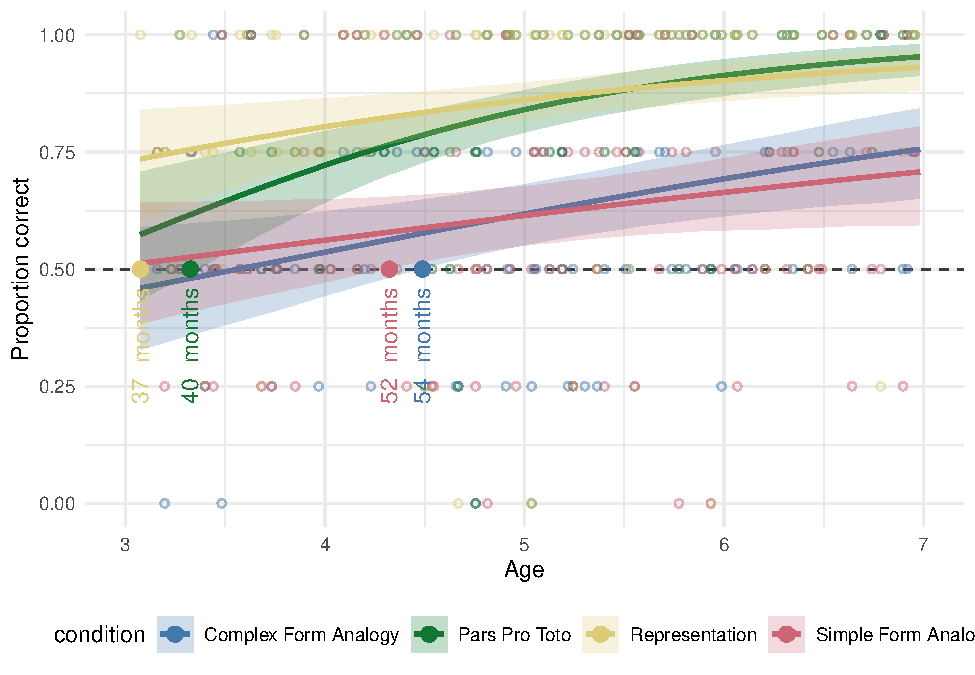
\includegraphics{symlit_rep_manuscript_files/figure-latex/S1_bayes_plot_no_facets-1.pdf}

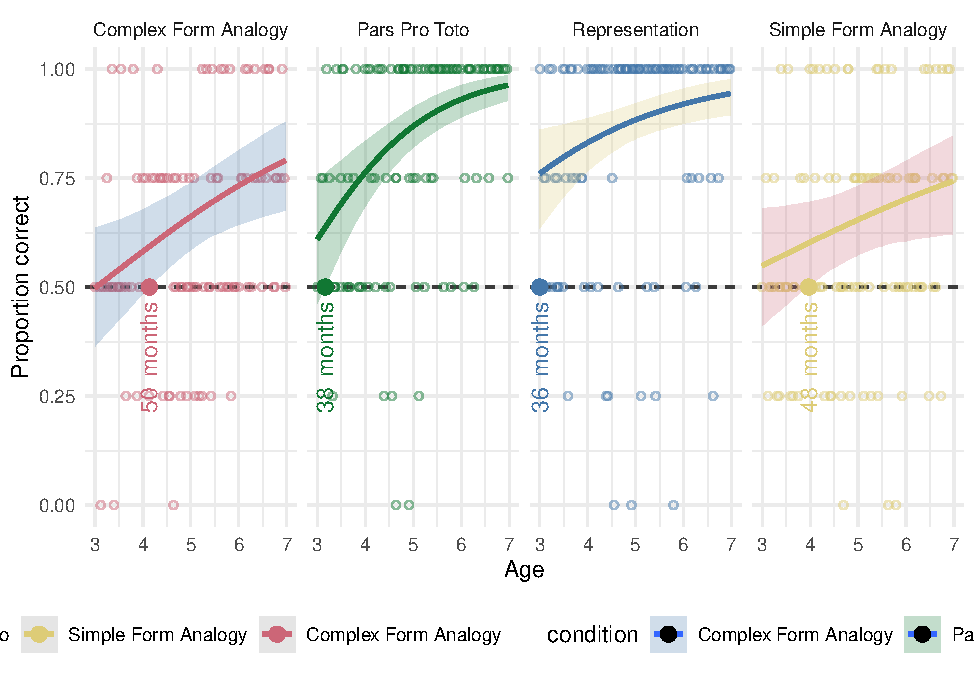
\includegraphics{symlit_rep_manuscript_files/figure-latex/S1_bayes_plot-1.pdf}

\st{Lorem ipsum dolor sit amet, consetetur sadipscing elitr, sed diam nonumy eirmod tempor invidunt ut labore et dolore magna aliquyam erat, sed diam voluptua. At vero eos et accusam et justo duo dolores et ea rebum. Stet clita kasd gubergren, no sea takimata sanctus est Lorem ipsum dolor sit amet. Lorem ipsum dolor sit amet, consetetur sadipscing elitr, sed diam nonumy eirmod tempor invidunt ut labore et dolore magna aliquyam erat, sed diam voluptua. At vero eos et accusam et justo duo dolores et ea rebum. Stet clita kasd gubergren, no sea takimata sanctus est Lorem ipsum dolor sit amet.}

\subsection{Study 2}\label{study-2}

\subsubsection{Participants}\label{participants-1}

A total of 99 three- to seven-year-old children (M = 60.04 months, SD = 13.69 months, range 36 - 83 months; 49 female) participated. In addition, 15 children (7 female) were tested but excluded from analysis for failing familiarization (N = 10), being fussy (N = 2), not being fluent in German (N = 1) or due to technical issues (N = 2).

\subsubsection{Materials}\label{materials}

\subsubsection{Data analysis}\label{data-analysis}

Notation
Evaluation of model Stability

\subsubsection{Results}\label{results-1}

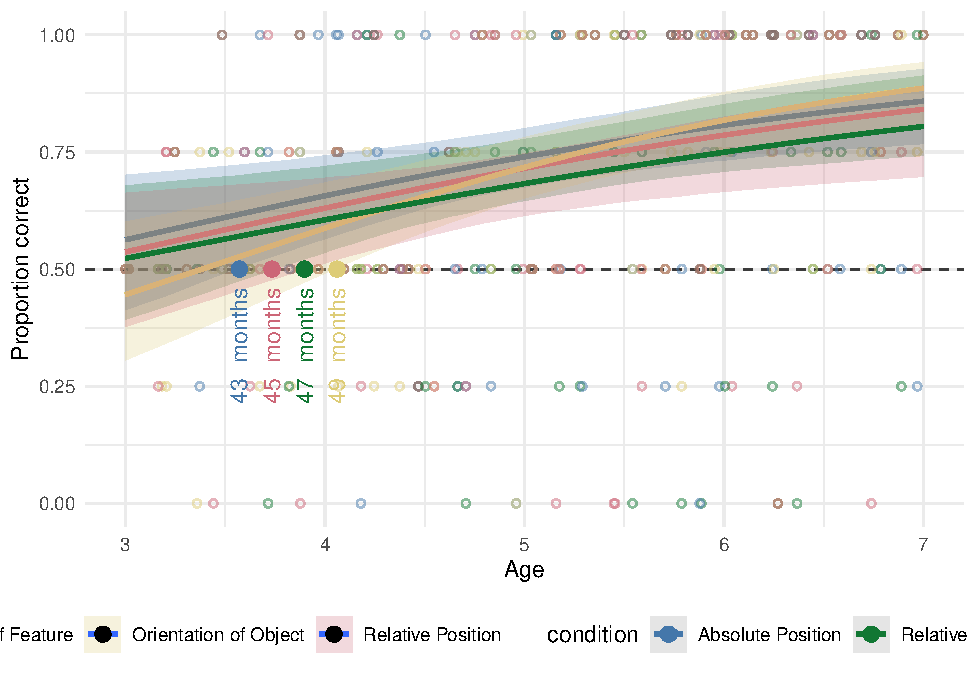
\includegraphics{symlit_rep_manuscript_files/figure-latex/S2_bayes_plot-1.pdf}

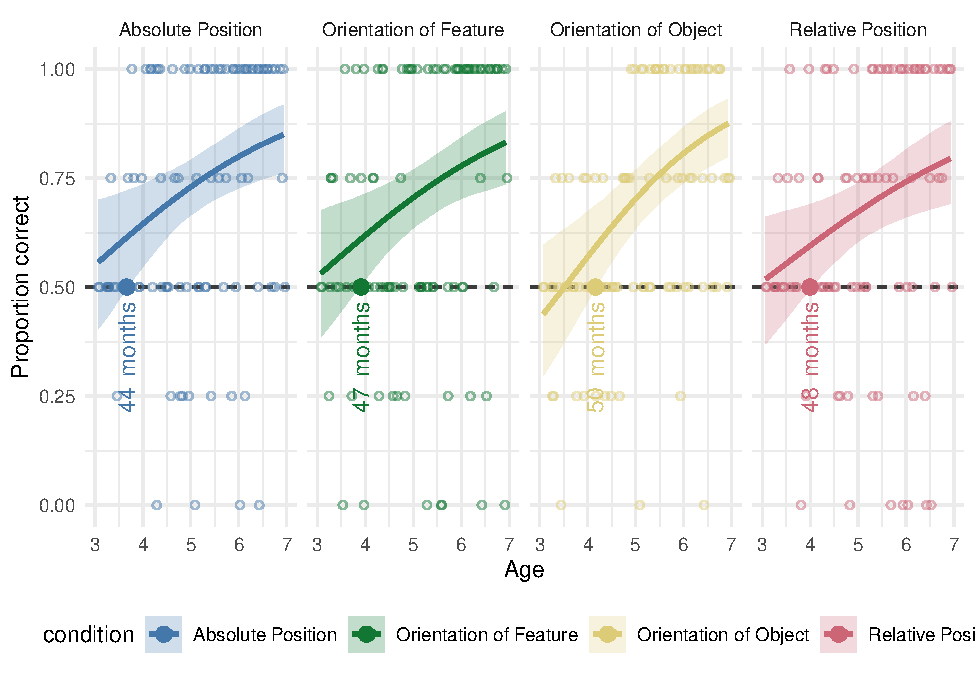
\includegraphics{symlit_rep_manuscript_files/figure-latex/S2_mixbayes_plot-1.pdf}

\subsection{Study 3}\label{study-3}

General note on the aim of the investigation

\subsubsection{Participants}\label{participants-2}

A total of 99 three- to seven-year-old children (M = 59.88 months, SD = 13.44 months, range 36 - 83 months; 55 female) participated. In addition, 23 children (7 female) were tested but excluded for low performance during familiarization (N = 12), for not completing at least eight out of 16 test trials (N = 1), or being fussy (N = 3). Another 4children were excluded due to language problems or technical issues (N = 3).

\subsubsection{Materials}\label{materials-1}

\subsubsection{Analysis}\label{analysis}

Trails
Notation
Model Evaluation

\subsubsection{Results}\label{results-2}

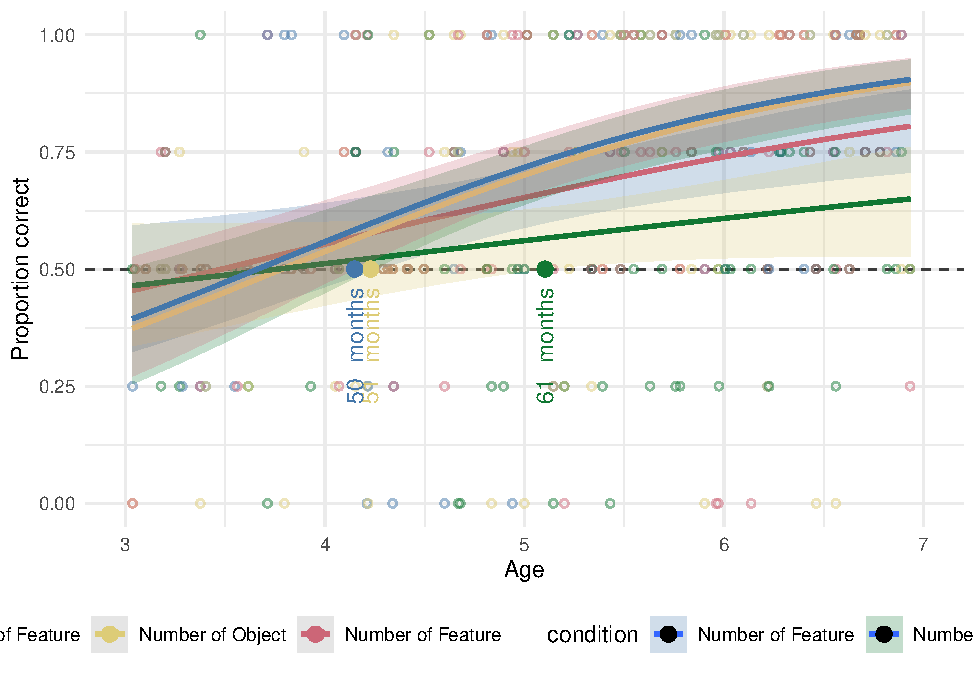
\includegraphics{symlit_rep_manuscript_files/figure-latex/S3_bayes_plot-1.pdf}

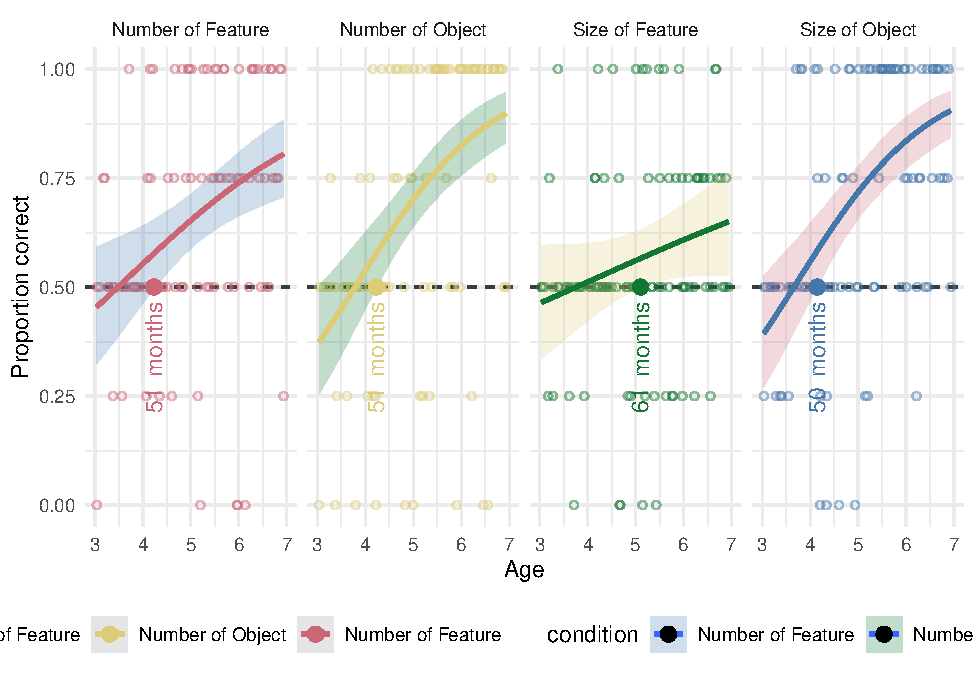
\includegraphics{symlit_rep_manuscript_files/figure-latex/S3_mixbayes_plot-1.pdf}

Lorem ipsum dolor sit amet, consetetur sadipscing elitr, sed diam nonumy eirmod tempor invidunt ut labore et dolore magna aliquyam erat, sed diam voluptua. At vero eos et accusam et justo duo dolores et ea rebum. Stet clita kasd gubergren, no sea takimata sanctus est Lorem ipsum dolor sit amet. Lorem ipsum dolor sit amet, consetetur sadipscing elitr, sed diam nonumy eirmod tempor invidunt ut labore et dolore magna aliquyam erat, sed diam voluptua. At vero eos et accusam et justo duo dolores et ea rebum. Stet clita kasd gubergren, no sea takimata sanctus est Lorem ipsum dolor sit amet.

\section{Additional Analyses}\label{additional-analyses}

possible add-ons
- a model including all conditions
- comparing difficulty across items and tasks
- evaluating manipulations such as complex/simple;
- reaction time analyses

Additional Analyses:

object vs feature
- orfe vs orob
- sife vs siob
- nufe vs nuob

round vs angular
- Study One Study1 - cue A = rund, cue B eckig \ldots if one of them is easier

Reaction Times
just reaction times and perc correct across aged

\section{General Discussion}\label{general-discussion}

Overview

Main Finding

Strengths and Implications

Limitations

\section{Conclusion}\label{conclusion}

Lorem ipsum dolor sit amet, consetetur sadipscing elitr, sed diam nonumy eirmod tempor invidunt ut labore et dolore magna aliquyam erat, sed diam voluptua. At vero eos et accusam et justo duo dolores et ea rebum. Stet clita kasd gubergren, no sea takimata sanctus est Lorem ipsum dolor sit amet.

\newpage

\section{References}\label{references}

\phantomsection\label{refs}
\begin{CSLReferences}{1}{0}
\bibitem[\citeproctext]{ref-bohn2019young}
Bohn, M., Kachel, G., \& Tomasello, M. (2019). Young children spontaneously recreate core properties of language in a new modality. \emph{Proceedings of the National Academy of Sciences}, \emph{116}(51), 26072--26077.

\end{CSLReferences}

\newpage

\appendix


\section{Participants and Exclusions}\label{participants-and-exclusions}

Data collection aimed at testing two children per month of age between the third and seventh birthday for a minimum of 96 children per study. For an overview of the sample distribution, please see figure \ref{fig:suppl-participants-dots}.

\begin{figure}

{\centering 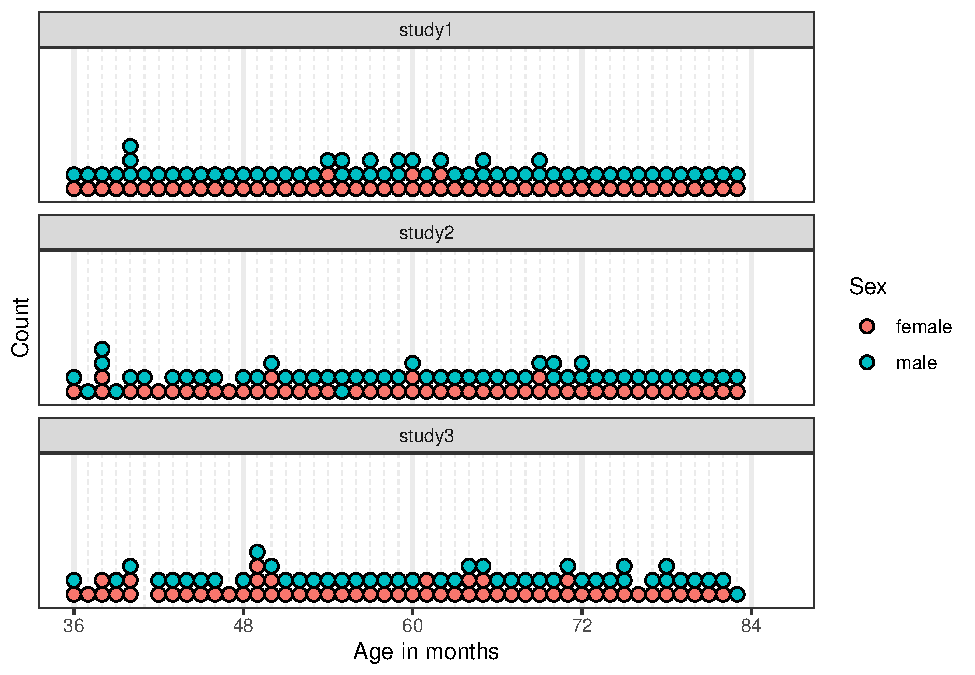
\includegraphics{symlit_rep_manuscript_files/figure-latex/suppl-participants-dots-1} 

}

\caption{Illustration of participants across the age range.}\label{fig:suppl-participants-dots}
\end{figure}

The total number of participants in all three studies comprises XX children. In addition, XX children were tested but not included in the data set due to XXXXXXXX. For an overview of how the respective exclusions are distributed across the age range, please see figure \ref{fig:suppl-drops-dots}. Exclusions due to low performance during familiarization occured almost exclusively between the third and fourth birthday. All other exclusion criteria appear to be randomly distributed across the age range.

\begin{verbatim}
## Warning: The `size` argument of `element_line()` is deprecated as of ggplot2 3.4.0.
## i Please use the `linewidth` argument instead.
## This warning is displayed once every 8 hours.
## Call `lifecycle::last_lifecycle_warnings()` to see where this warning was
## generated.
\end{verbatim}

\begin{figure}

{\centering 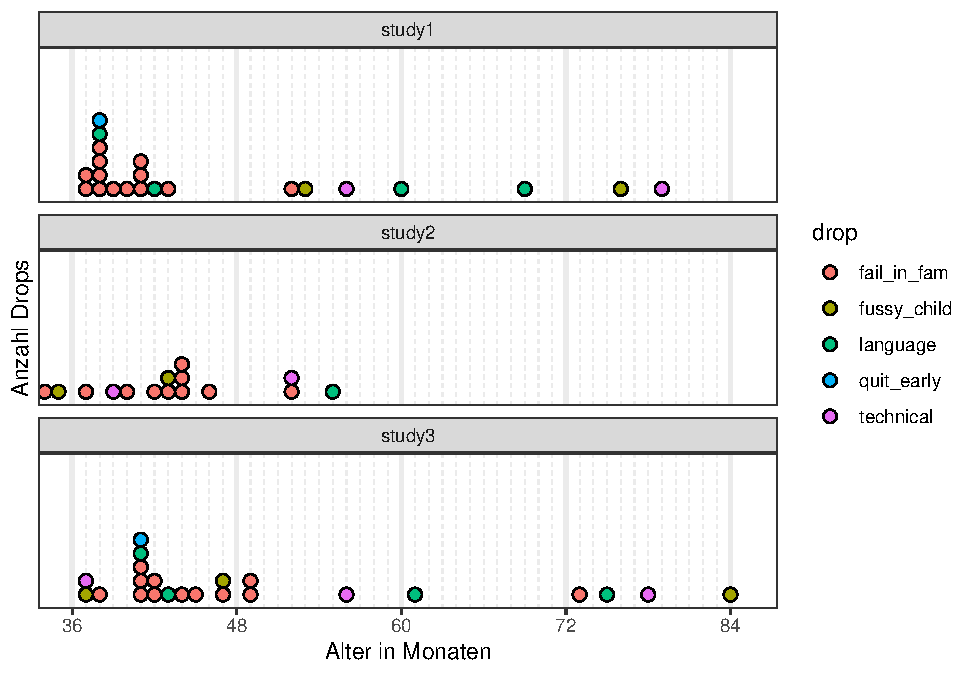
\includegraphics{symlit_rep_manuscript_files/figure-latex/suppl-drops-dots-1} 

}

\caption{Illustration of exclusions across the age range.}\label{fig:suppl-drops-dots}
\end{figure}

\section{Stimulus Material}\label{stimulus-material}

Additional Tables and illustrations for the convenience of the reader. Add illustrations they said; it will add value they said.

\subsection{Study 1}\label{study-1-1}

Additional Tables and illustrations for the convenience of the reader. Add illustrations they said; it will add value they said.

\subsection{Some graphic}\label{some-graphic}

\begin{figure}

{\centering 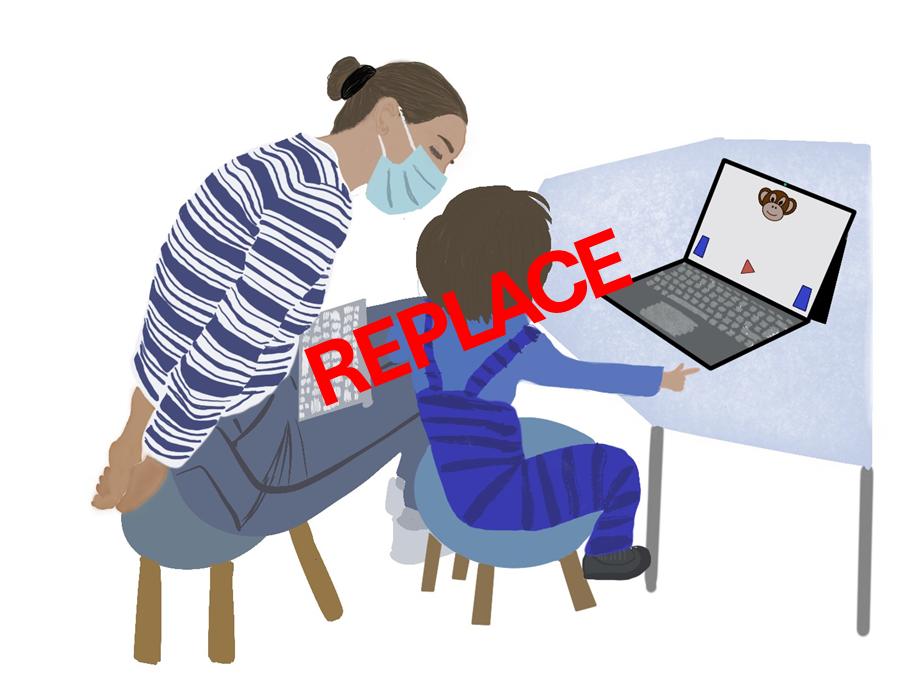
\includegraphics{../illustrations/Symlit_Rep_Setup} 

}

\caption{Check this out}\label{fig:suppl-setup3}
\end{figure}

\subsection{Study 2}\label{study-2-1}

Additional Tables and illustrations for the convenience of the reader. Add illustrations they said; it will add value they said.

\subsection{Some graphic}\label{some-graphic-1}

\begin{figure}

{\centering 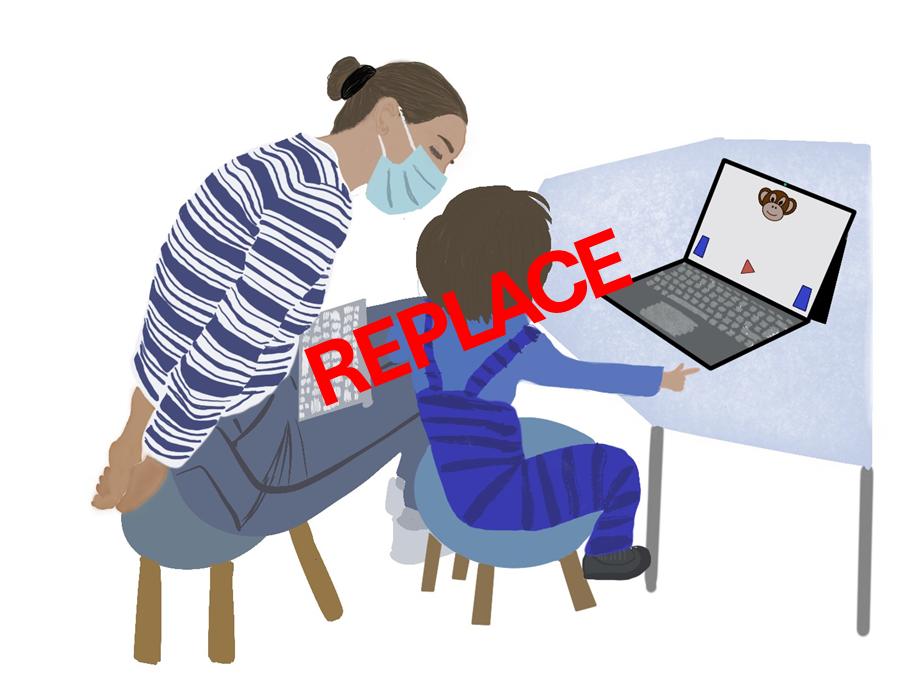
\includegraphics{../illustrations/Symlit_Rep_Setup} 

}

\caption{Check this out}\label{fig:suppl-setup4}
\end{figure}

\subsection{Study 3}\label{study-3-1}

Additional Tables and illustrations for the convenience of the reader. Add illustrations they said; it will add value they said.

\subsection{Some graphic}\label{some-graphic-2}

\begin{figure}

{\centering 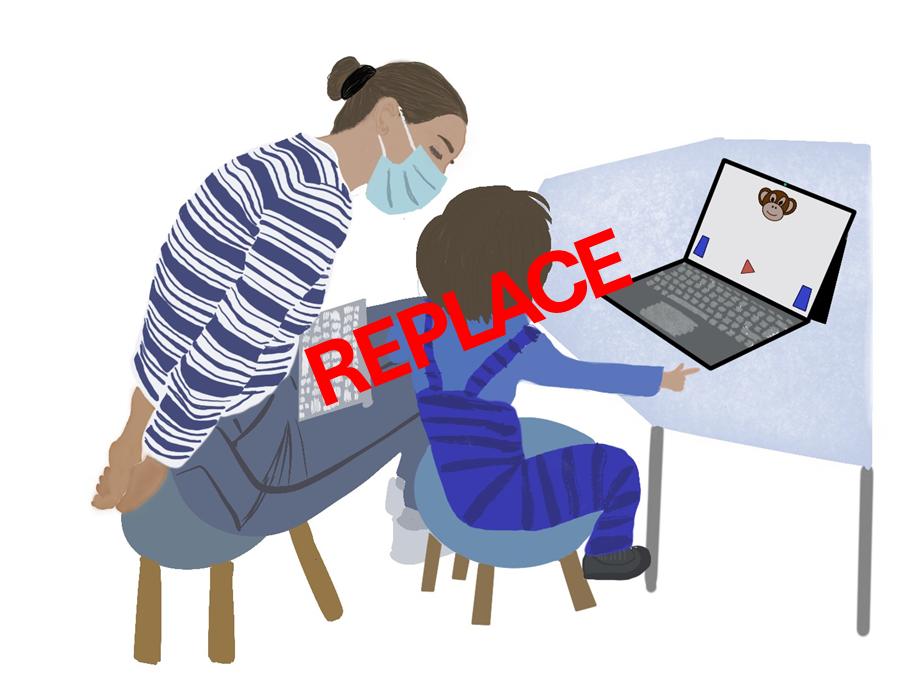
\includegraphics{../illustrations/Symlit_Rep_Setup} 

}

\caption{Check this out}\label{fig:suppl-setup5}
\end{figure}

\section{Descriptive Statistics}\label{descriptive-statistics}

Additional Tables and illustrations for the convenience of the reader. Add illustrations they said; it will add value they said.

\subsection{Study 1}\label{study-1-2}

Additional Tables and illustrations for the convenience of the reader. Add illustrations they said; it will add value they said.

\subsection{Study 2}\label{study-2-2}

Additional Tables and illustrations for the convenience of the reader. Add illustrations they said; it will add value they said.

\subsection{Study 3}\label{study-3-2}

Additional Tables and illustrations for the convenience of the reader. Add illustrations they said; it will add value they said.


\end{document}
